\documentclass{article}
\usepackage[utf8]{inputenc}

\title{Comp 150 Probabilistic Robotics Homework 1: Kalman Filter}
\author{James Staley}
\date{\vspace{-2em}}

\usepackage{natbib}
\usepackage{graphicx}
\usepackage{eucal}
\usepackage{url}

\begin{document}

\maketitle
{\bf Question 1.1}: what is the minimal state vector for the Kalman filter so that the resulting system is Markovian?\\

The minimal state vector holds the position and velocity of the system: $x = \{p_n, v_n\}$ where $n$ is the number of tracked dimensions. Position and velocity depend on the history of the system, and the condition probability distribution of future states depends on only these two variables. The acceleration does not need to be included because it's a random variable and doesn't depend on time or any other variable. 

{\bf Question 1.2}: Design the state transition probability function $p(x_t | u_t, x_{t-1})$. The transition function should contain linear matrices $A$ and $B$ and a noise covariance $R$.\\

The state transition probability function gives the liklihood of being in state $x_t$ given the previous state $x_{t-1}$ and the command signal $u_t$. The Kalman Filter models all uncertainty as gaussian noise. So the new state $x_t$ is actually the mean of a gaussian distribution given by eqn. \ref{position_update}, where $A$ is a matrix that converts the previous state forward by one timestep, and $B$ is a matrix that converts the command signal to changes in state. The covariance of the gaussian distribution is given in eqn. \ref{covariance_update}, where the noise matrix $R$ is constructed from the variance of the expected noise, and the vector $G$ which describes how the random variable (acceleration in this case) will affect each state variable (eqn. \ref{R_calc}). The state transition probability function is given by the mean $x_t$ and covariance $\Sigma_t$. The state is initialized to zero while the covariance is initialized to an identity matrix. The values for $A$, $B$, and $G$ can be found in the top of the attached python file.

\begin{equation}\label{position_update}
    x_t = A_t x_{t-1} + B_t u_t
\end{equation}

\begin{equation}\label{covariance_update}
    \Sigma_t = A_t \Sigma_{t-1} A^T_t + R_t
\end{equation}

\begin{equation}\label{R_calc}
    R = \sigma^2 G G^T
\end{equation}

{\bf Question 1.3 + 1.4}: Implement the state prediction step of the Kalman filter, assuming that at time $t = 0$, we start at rest, i.e., $x_t = \dot{x}_t = \ddot{x}_t = 0.0$. Use your code to calculate the state distribution for times $t = 1, 2, \ldots, 5$.\\
For each value of $t$ in the previous question, plot the joint posterior over $x$ and $\dot{x}$ in a diagram where $x$ is the horizontal and $\dot{x}$ is the vertical axis. For each posterior, you are asked to plot the uncertainty ellipse which is the ellipse of points that are one standard deviation away from the mean. Some additional information about uncertainty ellipses and how to calculate them using MATLAB or C++ can be found here: \url{http://www.visiondummy.com/2014/04/draw-error-ellipse-representing-covariance-matrix/}.

I the predicted position of the sailboat at each timestep and drew an ellipse axis aligned with the eigenvectors of the covariance matrix to show the uncertainty in position and velocity. The size of the ellipse corresponds to roughly one-standard deviation of uncertainty. I could not find a chi-squared table value needed for 1 standard deviation (n where $1-n = 0.68$), so I used 0.75 as an approximation when calculating the size of the ellipse.

\begin{figure}[h]
    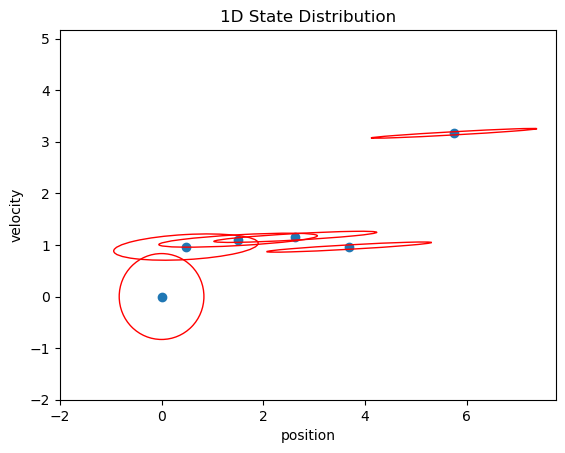
\includegraphics[width=8cm]{conf_ellipses.png}
    \centering
    \caption{Five timesteps of prediction for the motion model with multivariate gaussian noise. Each sample has a confidence ellipse that shows how uncertain the estimate of position and velocity are for that prediction.}
\end{figure}

The above figure shows how uncertainty in the predictions evolves over time. Before any updates our uncertainty is a circle around our first point, but as we forward predict and incorporate multivariate noise the uncertainty stretches over position and rotates. We have much more uncertainty in our position than we do in our velocity because our position is influenced by the noise in velocity in addition to the noise from acceleration. Its two steps down the chain.

\section{Kalman Filter: Measurement}

Prediction alone will result in greater and greater uncertainty as time goes on. Fortunately, your sailboat has a GPS sensor, which in expectation, measures the true position. However, the measurement is corrupted by Gaussian noise with covariance $\sigma_{gps}^2 = 8.0$.\\

{\bf Question 2.1}: Define the measurement model. You will need to define matrices $C$ and $Q$. \\

{\bf Question 2.2}: Implement the measurement update. Suppose at time $t = 5$, we query our sensor for the first time to obtain the measurement $z = 10$. State the parameters of the Gaussian estimate before and after incorporating the measurement. Afterwards, implement the sensor modal to randomly sample the true position, corrupted with noise $\sigma_{gps}^2$. \\

{\bf Question 2.3}: All of a sudden, the sky gets cloudy which may cause the sensor to fail and not produce a measurement with probability $p_{gps-fail}$. For three different values of this probability (e.g., 0.1, 0.5, and 0.9), compute and plot the expected error from the true position at time $t = 20$. You may do so by running up to $N$ simulations and use the observed errors to obtain the expected error empirically.  

\section{Extra Credit}

Now, formulate both the prediction and measurement steps in the 2-D case. Construct a plot showing the true position and the position tracked by the Kalman filter over the first 30 time steps. \\

\noindent {\bf What to turn in:} A PDF document with the answers to the questions, along with the code implementation and a README file that describes what to run in order to get the results in your PDF. You can use a language of your choice. 


%\bibliographystyle{plain}
%\bibliography{references}
\end{document}
